\documentclass[a4paper, 12pt]{article}

\usepackage{amsmath}
\usepackage{amssymb}
\usepackage{cases}
\usepackage{color}
\usepackage{empheq}
\usepackage[english]{babel}
\usepackage{enumerate}
\usepackage{enumitem}
\usepackage{epstopdf}
\usepackage{fancyhdr}
\usepackage{float}
\usepackage{gensymb}
\usepackage{graphicx}
\usepackage{hyperref}
\usepackage{ifthen}
\usepackage{listings}
\usepackage[miktex]{gnuplottex}
\usepackage{subcaption}
\usepackage{subfiles}
\usepackage{textcomp}
\usepackage{tikz}
\usepackage[top=0.5in,bottom=0.5in,left=0.5in,right=0.5in]{geometry}
\usepackage[utf8]{inputenc}

\usetikzlibrary{shapes,arrows,positioning,shadows,calc}


\definecolor{orange}{rgb}{1,0.5,0}
\definecolor{lightgray}{rgb}{.9,.9,.9}
\definecolor{xml_keyword}{rgb}{0.37, 0.08, 0.25}
\definecolor{xml_string}{rgb}{0.06, 0.10, 0.98}
\definecolor{xml_comment}{rgb}{0.12, 0.38, 0.18}
\definecolor{xml_doc}{rgb}{0.25,0.35,0.75}

\newcommand{\norm}[1]{\left\lVert#1\right\rVert}

\graphicspath{{./images/}}


\title{\textbf{Introduction to Neuroinformatics} \\Summary of the lectures
2018\\\normalsize Version 4.0 \\
for internal use by students attending the lecture only}

\author{
\texttt{Initial Version 2012}\\
	Benjamin Ellenberger
\and
\texttt{Revision 2013}\\
	Joachim Ott\\Dora Sumislawska
\and
\texttt{Revision 2014}\\
	Fabian Tschopp
\and
\texttt{Revision 2018}\\
	Vanessa Leite}

\date{}


\begin{document}
\maketitle
\newpage
\tableofcontents
\newpage

\newpage

\subfile{01-introduction.tex}

\subfile{02-nervous-system-organization.tex}

\subfile{03-membrane-potential.tex}

\subfile{04-passive-membrane-properties.tex}

\subfile{05-action-potential.tex}

\subfile{06-rate-event-code.tex}

\subfile{07-synapse-I.tex}

\subfile{08-synapse-II.tex}

\subfile{09-plasticity.tex}

\subfile{10-neuromorphic.tex}

\subfile{11-gates.tex}

\subfile{12-perceptron.tex}

\newpage

\section{Feed-Forward Networks}
\begin{itemize}[noitemsep,nolistsep]
	\item Multiple layers of neurons with a certain number of inputs and outputs.
	\item Every laxer of nodes feeds the next layer with inputs.
	\item There is an input and an output layer with hidden layers in between.
\end{itemize}
\begin{figure}[H]
	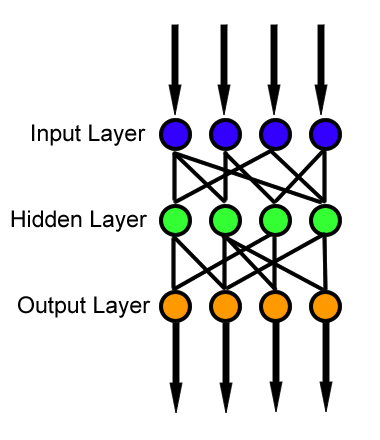
\includegraphics[width=0.25\textwidth]{Feed_forward_neural_net.png}
\end{figure}

\subsection{Backpropagation and Error function}
\begin{itemize}[noitemsep,nolistsep]
	\item The inputs and desired outputs are given as $S=\{(x,d)^1,\ldots,(x,d)^l\}$.
	\item The error function is given as $E(S) = \sum_i\frac{1}{2}||y(x^i)-d^i||^2$.
	\item The output is a non-linear transformation $y=f(a)$.
	\item $f(a)$ is the activation function, which is usually a sigmoid function.
	\item The error function for a single training sample is $E(S)=\frac{1}{2}(f(x_1w_1+x_2w_2+w_0)-d)^2$.
	\item The output of a simple network is for example $y(x_1,x_2,x_3)=f(x_1w_{21}+f(x_2w_{11}+x_3w_{12}+w_{10})w_{22}+w_{20})$.
	\item $\frac{\partial E(w_1,w_2,w_0)}{\partial w_1}=(f(x_1w_1+x_2w_2+w_0)-d)\cdot f'(x_1w_1+x_2w_2+w_0)\cdot x_1$.
	\item $\frac{\partial E(w_1,w_2,w_0)}{\partial w_2}=(f(x_1w_1+x_2w_2+w_0)-d)\cdot f'(x_1w_1+x_2w_2+w_0)\cdot x_2$.
	\item $\frac{\partial E(w_1,w_2,w_0)}{\partial w_0}=(f(x_1w_1+x_2w_2+w_0)-d)\cdot f'(x_1w_1+x_2w_2+w_0)$.
	\item The error terms travel backwards through the network and get multiplied with the derivative of the activation function of that input. Multiple error terms can just be added up.
	\item The partial derivative of the error $E$ term in relation to the weight $w$ to be adjusted can be added to the weight in order to learn. An additional weighting factor can be added.
\end{itemize}

\section{Signal Propagation in a Network}
\subsection{Avalanche Model}
\begin{itemize}[noitemsep,nolistsep]
	\item For example needed with sensory neurons, as smalls ignals have to be amplified in order to be detectable by the superior areas.
	\item No recurrent connections or risk of positive feedback with risk of explosion.
	\item $(pn)^2$ active neurons per layer. $p$ is a probability and $n$ is the number of neurons that every next layer has more than the previous ones. One neuron from the last layer is connected with $n$ from the next one.
\end{itemize}

\subsection{Synfire Chain}
\begin{itemize}[noitemsep,nolistsep]
	\item The synfire chain is a feedforward structure.
	\item Synchrony is the most important factor for the transmission of the signal.
	\item Noise is important: The chain is usually embedded in a larger network to transmit information. Introducing noise avoids that large-scale synchronization of neuronal firing contaminates the whole network.
\end{itemize}

\subsection{Divergence, convergence}
\begin{itemize}[noitemsep,nolistsep]
	\item A connection is said to be converging if a neuron receives input from several other neurons.
	\item A connection is said to be diverging if a neuron projects to several other neurons.
\end{itemize}

\section{Interacting Neural Populations}
\begin{itemize}[noitemsep,nolistsep]
	\item Neurons can represent information through population codes.
	\item Neurons are tuned to preferred stimuli.
	\item Information is represented by the pattern of activity in a neural population.
	\item Each neuron has a preferred input, for example orientation, that it responds to. The neuron is tuned to that value.
	\item Not every neuron shows clear tuning curves.
	\item Neurons usually do not only respond to their preferred stimulus, but also with decaying strength to close ones.
\end{itemize}

\begin{figure}[H]
	\centering
	\begin{subfigure}[b]{0.3\textwidth}
		\centering
		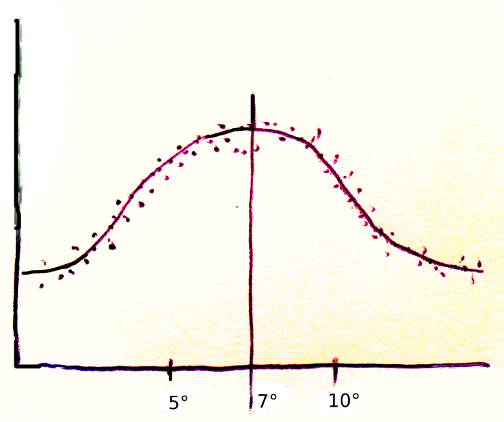
\includegraphics[width=\textwidth]{one-cell-tuning-curve.png}
		\caption{Tuning curve of one cell}
	\end{subfigure}%
	~
	\begin{subfigure}[b]{0.3\textwidth}
		\centering
		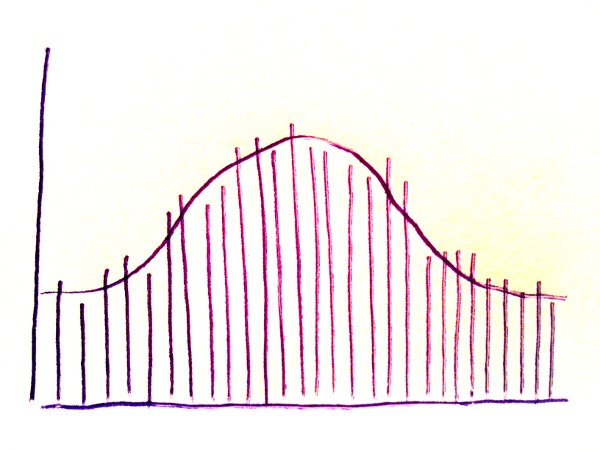
\includegraphics[width=\textwidth]{cell-order.png}
		\caption{Cells ordered by response to $20^\circ$}
	\end{subfigure}
	~ 
	\begin{subfigure}[b]{0.3\textwidth}
		\centering
		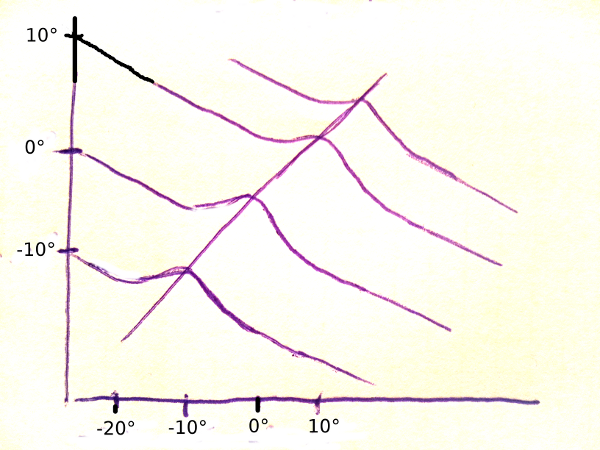
\includegraphics[width=\textwidth]{3D-visualisation.png}
		\caption{3D visualization of cell's response to different degrees}
	\end{subfigure}
\end{figure}

\begin{figure}[H]
	\centering
	\begin{subfigure}[b]{0.5\textwidth}
		\centering
		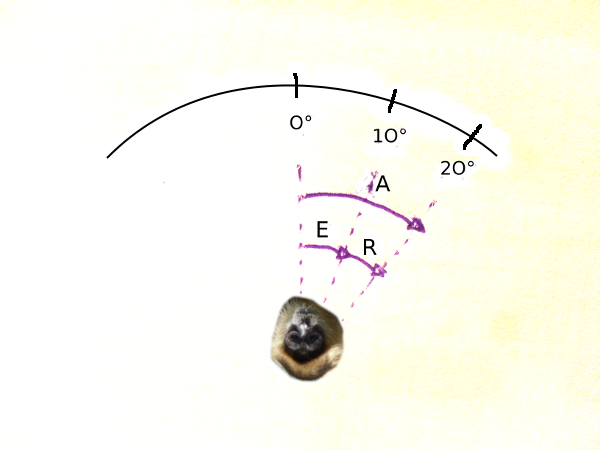
\includegraphics[width=\textwidth]{ape-picture.png}
		\caption{Monkey holding gaze fixed on point $10^\circ$ and light falling in from $20^\circ$}
	\end{subfigure}%
	~
	\begin{subfigure}[b]{0.5\textwidth}
		\centering
		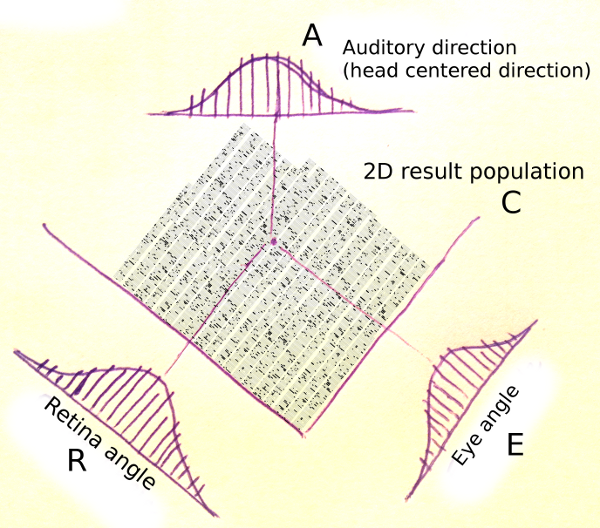
\includegraphics[width=\textwidth]{Retina-Eye-Auditory.png}
		\caption{Visualization of Retina angle ordering cell set R, Eye angle ordering set E,2D result population C and auditory direction set A.}
	\end{subfigure}
\end{figure}

\begin{figure}[H]
	\centering
	\begin{subfigure}[b]{0.3\textwidth}
		\centering
		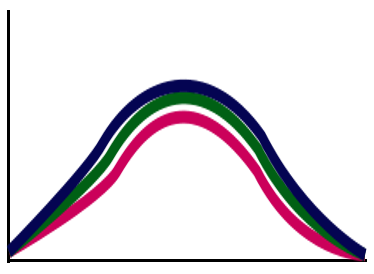
\includegraphics[width=\textwidth]{Cell-A.png}
		\caption{Cell A $\in$ R}
	\end{subfigure}%
	~
	\begin{subfigure}[b]{0.3\textwidth}
		\centering
		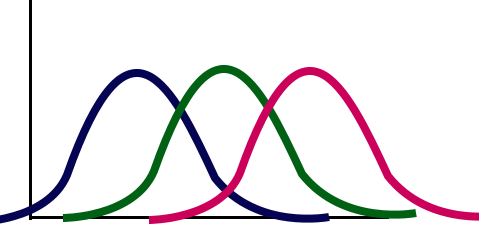
\includegraphics[width=\textwidth]{Cell-B.png}
		\caption{Cell B $\in$ A}
	\end{subfigure}
	~ 
	\begin{subfigure}[b]{0.3\textwidth}
		\centering
		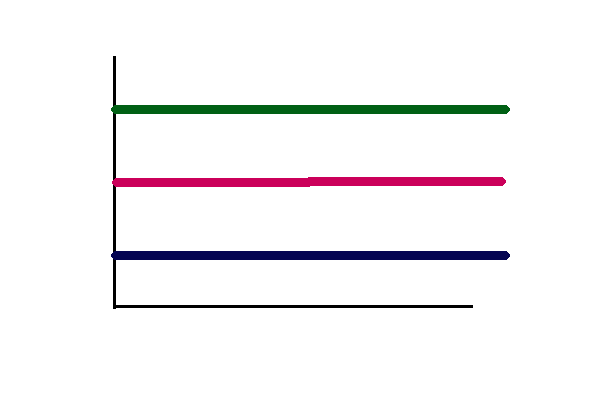
\includegraphics[width=\textwidth]{Cell-C.png}
		\caption{Cell C $\in$ E}
	\end{subfigure}
\end{figure}

\begin{figure}[H]
	\centering
	\begin{subfigure}[b]{0.3\textwidth}
		\centering
		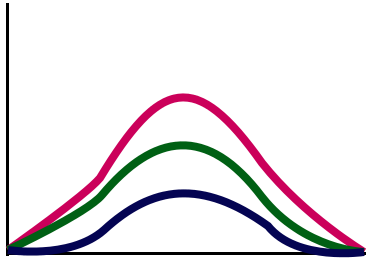
\includegraphics[width=\textwidth]{Cell-D.png}
		\caption{Cell D $\in$ C}
	\end{subfigure}%
	~
	\begin{subfigure}[b]{0.3\textwidth}
		\centering
		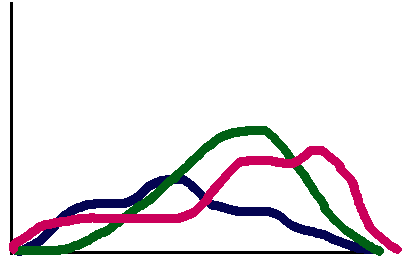
\includegraphics[width=\textwidth]{Cell-E.png}
		\caption{Cell E (Not every neuron shows clear tuning curves)}
	\end{subfigure}
\end{figure}

\newpage
\subsection{References}
The pictures used in this summary are from the following books and slide sets
and belong to their respective owners. In the context of the summary they are
used for educational purposes only.
\begin{itemize}
\item D. Purves et al.: Neuroscience. Fifth edition. Sinauer

\item Squire, Berg, Bloom, du Lac, Ghosh \& Spitzer: Fundamental Neuroscience. Elsevier

\item Eric Kandel et al.: Principles of Neural Science. Fifth edition.
McGraw-Hill 

\item Peter Dayan, L. F. Abbott: Theoretical Neuroscience, The MIT
Press

\item Christof Koch: Biophysics of Computation. Oxford University Press

\item John Nicholls et al.: From Neuron to Brain. Palgrave Macmillan

\item W. Gerstner et al.: Neuronal Dynamics. From Single Neurons to Networks and Models of Cognition. Cambridge University Press (2014).

\item Hertz, Krogh, Palmer: Introduction to the Theory of Neural Computation.
Westview Press

\item Bishop: Pattern Recognition and Machine Learning. Springer

\item The lecture slides of the Introduction to Neuroinformatics course of the
years 2012, 2013, 2014 and 2018.

\end{itemize}
\end{document}